\chapter{Flow-Limited Authorization for secret sharing}\label{ch:flaqrplus}
\section{Introduction}


An extension to \FLAQR\ adding support for simple secret sharing, and results demonstrating it preserves integrity and availability noninterference as well as our liveness theorem, despite introducing an additional source of failure due to mismatched shares (\ref{sec:SecretSharing}).

This paper is an expanded and updated version of an article previously published in the proceedings of the 35$^{th}$ Computer Security Foundations Symposium~\cite{flaqr}. This version adds support for secret sharing (Section~\ref{sec:SecretSharing}) and extensions of our previous results that demonstrate these new terms neither impact integrity and availability noninterference, nor majority liveness, despite introducing an additional source of failure. In addition, we corrected a minor issue in the original blame semantics, and include complete rule sets and proofs for our formalization and theoretical results.

\section{Secret sharing with \FLAQR} \label{sec:SecretSharing}
Secret sharing is a cryptographic mechanism used in several distributed systems protocols
such as oblivious transfer, multiparty communication, and Byzantine agreement. 
In this section we extend \FLAQR\ with two new language constructs to support secret sharing. 
We call this extended version of our programming model \FLAQRp.
%\subsection{\textbf{Secret sharing}} 
Secret sharing is a process of splitting 
a secret into $n$ shares
and distributing the shares among $n$ hosts (or principals in our setting). 
When an adequate number of hosts, say $t$, combine their respective 
shares, the secret is reconstructed~\cite{Shamir79,secshr}.
Sometimes this process is referred as \emph{(t,n)-threshold} 
secret sharing scheme \cite{Shamir79, tnsecshr}, 
i.e. a quorum of $t$ hosts (where $1 < t \leq n$) out of 
those $n$ hosts need to combine their shares to retrieve the initial secret 
value. With $(t-1)$ or fewer shares, adversaries learn nothing about the secret.

Secret sharing is most commonly described in terms of a mathematical 
polynomial, say $p(x)$, of degree $(t-1)$, $p(0)$ being the secret value~\cite{Shamir79}. 
The polynomial's values at $n$ different co-ordinates are distributed as the secret shares, 
and by knowing $t$ of these values one 
can reconstruct\footnote{Typically using Lagrange interpolation~\cite{secshr}.}
the polynomial and find the secret value $p(0)$. 

For simplicity, we extend \FLAQR\ to support \emph{(2,2)-threshold}
secret sharing, but later sketch how support for
\emph{(t,n)-threshold} secret sharing where $2 < n$ and $t < n$ would be
straightforward. We model secret shares abstractly using a value sealed by
new kinds of principals $k.L$ and $k.R$. We call $k$ a \emph{key principal}
because, unlike the principals in $\P$, a new, unique key principal $k$ is created
each time secret shares are created. In contrast, the principals in $\P$ are statically
known. 

The principals $k.L$ and $k.R$ represent the two associated shares of the key principal $k$.
We will be referring to \emph{(2,2)-threshold} secret sharing
simply as \emph{(2,2)} secret sharing in the following sections.


\subsection{Motivating example of secret sharing : password splitting.}\label{sec:motivsecshr}
Figure \ref{fig:secshrfig} presents a simple \emph{(2,2)} secret sharing example and the corresponding 
pseudocode is shown in Figure \ref{fig:motivatesecshr}.
A (secret) password "s" belongs to "bob" who wants keep a backup of it. 
Bob creates two secret-shares of "s" as "s1" and "s2" and sends them to "alice" and "carol" respectively. That is, anyone who wants to get access to "s" has to either get it directly from "bob", or needs to get both "s1" and "s2" from "alice" and "carol" and reproduce it. 
Later, "dave" fetches the secret shares from "alice" and "carol" and combines them to 
produce the password "s".


An advantage of secret sharing is that it permits the secure
transmission of secrets without requiring key distribution or
public-key infrastructure (PKI). Instead, any party who possesses $t$
shares may recover the secret. This can also be a liability, however,
since an adversary needs to only obtain the shares to access the secret,
too.  Thus, considering the flow of shares between principals is
central to the security of a secret sharing scheme.  In the example in
Figure~\ref{fig:motivatesecshr}, "alice" and "carol" are unable to access
the secret because they only possess a single share, but a coding error
could transmit both shares to "alice" or "carol", obviating the
cryptographic protection.  For this reason, embedding secret sharing
in a language like \FLAQR\ makes sense because the type system ensures
the code only permits authorized flows.


\begin{figure*}
\centering 
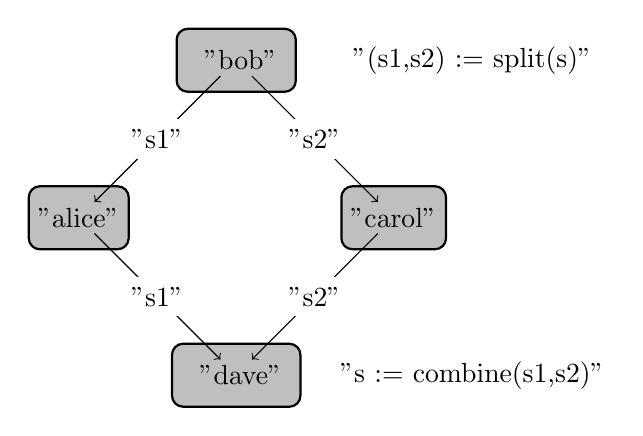
\begin{tikzpicture}
[
mysquare/.style={rectangle, draw=black, fill=gray!50, thick, minimum size=8mm, rounded corners},
tbox/.style={rectangle, draw=white, fill=white, thick, minimum height=0.2cm},
]
\node at (0,0) [mysquare]      (ball3)     {~~"bob"~~};
\node at (3,0) [tbox]      (ball3)     {"(s1,s2) := split(s)"};
\node at (-2,-2) [mysquare]      (ball3)     {"alice"};
\node at (2,-2) [mysquare]      (ball3)     {"carol"};
\node at (0,-4) [mysquare]      (ball3)     {~~"dave"~~};
\node at (3,-4) [tbox]      (ball3)     {"s := combine(s1,s2)"};

\draw[->] (-0.2,-0.2) -- (-1.8,-1.8);
\node at (-1,-1) [tbox]      (ball3)     {"s1"};
\draw[->] (0.2,-0.2) -- (1.8,-1.8);
\node at (1,-1) [tbox]      (ball3)     {"s2"};
\draw[->] (-1.8,-2.2) -- (-0.2,-3.8);
\node at (-1,-3) [tbox]      (ball3)     {"s1"};
\draw[->] (1.8,-2.2) -- (0.2,-3.8);
\node at (1,-3) [tbox]      (ball3)     {"s2"};
%\draw [->,red, very thick] (b4.east) to [out=10,in=330] (b1.east) ;
\end{tikzpicture}
\caption{Not working alice}
%\caption{Overview of $(2,2)$ secret sharing: "bob" shares his secret shares with "alice" and "carol". Later, "alice" and "carol" forward their respective shares to "dave". Finally, "dave" reproduces the initial secret "s" with the shares he received from "alice" and "carol".}
\label{fig:secshrfig}
\end{figure*}


\begin{figure*}
\centering 
\begin{lstlisting} 
splitCombinePassword():
  (s1,s2) := split(s) $@$ bob;$\label{ss:split}$
  send s1 to alice; $\label{ss:send1}$
  send s2 to carol;$\label{ss:send2}$
  con := func();$\label{ss:func}$ $\textcolor{blue}{\textup{// func() returns a bool}}$
  if(con)$\label{ss:ifs}$
    fetch s1 from alice;$\label{ss:get1}$
    fetch s2 from carol;$\label{ss:get2}$
    s' := combine(s1,s2) $@$ dave; $\label{ss:combine}$
  else return;
\end{lstlisting}
\caption{Creating two secret shares from a secret and then reconstructing the secret from the two secret shares using functions of a $(2,2)$ secret sharing protocol.}
\label{fig:motivatesecshr}
\end{figure*}


\subsection{$(2,2)$ secret sharing in \FLAQRp} \label{sec:secshrStart}

Our abstractions for secret sharing in \FLAQRp make use of the
$\retetav{\ell}{}$ term to represent sealed secret shares. 
However, aspects
of secret sharing schemes differ from the use of $\retetav{\ell}{}$ in prior
FLAC-based languages~\cite{jflac,dflate,nmifc}.  Here, in addition to the sealed values
generated by the $\returnp{\ell}$ term, sealed values may also
be created when splitting a secret into shares. In the previous approaches,
a value sealed by $\returnp{\ell}{}$
serves as a reasonable model for signed and encrypted values.  Specifically, the confidentiality component $\ell^{\confid}$ behaves like a public-key encrypted value: anyone can encrypt values at $\ell^{\confid}$, but only authorized parties (which
possess the associated private key) can distinguish the values protected at $\ell^{\confid}$.
Since $\returnp{\ell}{}$ can only be applied in contexts where $\pc \actsfor \ell^{\integ}$
(see \ruleref{UnitM}),
the integrity component behaves like a digitally signed value: only authorized
principals can cause a value to be signed with $\ell^{\integ}$ integrity, but anyone
can use high-integrity values.\footnote{There doesn't appear to be a natural cryptographic
  analog for the availability component.} Obviously then, enforcing these policies
cryptographically would require public-key infrastructure.

Secret sharing behaves differently from the above interpretations: rather
than authorization being based on possession of a long-lived private key (a reasonable
proxy for identity), secret sharing implicitly authorizes \emph{any party} possessing
$t$ shares. Therefore using identity-based principals such as \texttt{alice} or \texttt{bob}
is inappropriate since, even if a shared secret is intended for \texttt{alice},
anyone with $t$ shares will be able to distinguish the secret. Even \texttt{alice}
must have $t$ shares to access the secret. An abstraction for secret sharing should
capture this behavior, but doing so in \FLAQRp requires new concepts.

We extend the set of principals \P\ with new primitive principals $L$
and $R$ representing the left and right shares of our $(2,2)$ secret
sharing scheme. The set of all principals $\P$ for \FLAQRp is thus the
closure of the set $\N \cup \{\top, \bot, L, R\}$ over the same operations as
\FLAQR. In the following we are only interested in the confidentiality
projections $L^{\confid}$ and $R^{\confid}$, since secret sharing only
concerns enforcing the confidentiality of the secret.

Another aspect of secret sharing that departs from prior uses of FLAC
principals is that each time shares are created, they are protected by
a different secret.  Consequently, shares created from different
invocations cannot be mixed, even when the underlying value is the same.
For this reason, we define \emph{key principals}, a new type of principal
generated dynamically at runtime. For our purposes, each $k \in \keys$,
where $\keys$ is the set of all key principals, is equipped with a left
and right principal, $k.L^{\confid}$ and $k.R^{\confid}$. Importantly, since key principals
are generated dynamically, they are not directly representable statically.
The principals $L^{\confid}$ and $R^{\confid}$ are the static representation for the
left and right principals of any key principal, but the shares of different
key principals cannot be distinguished at the type level.


\subsection{Semantics and types for secret sharing}

\begin{figure*}
\begin{flushleft}
\begin{mathpar}

\erule{E-Split}{k \text{ is fresh}}
{\splits{\ell}{v}}{\pair{\returnv{k.L^{\confid} \wedge \ell}{v}}{\returnv{k.R^{\confid} \wedge \ell}{v}}} 

\erule{E-Combine}{}
{\comb{x}{\pair{\returnv{k.L^{\confid}\wedge \ell}{v}}{\returnv{k.R^{\confid}\wedge \ell}{v}}}{pc}{e}}{\subst{e}{x}{v}}
%{\comb{x}{\pair{\returnv{k.L\wedge \ell}{v}}{\returnv{k.R \wedge \ell}{v}}}{\pc}{}}{}
%{\returnv{\ell}{x}}}{y}
%{\returnv{\ell}{v}}

\end{mathpar}
\end{flushleft}
\caption{\FLAQRp semantics for secret sharing (splitting secrets and combining shares).}
\label{fig:secShSem}
\end{figure*}

\begin{figure*}
\begin{mathpar}

\Rule{Split}
{
\TValGpcw{e}{\tau} \\
\rafjudge{\Pi}{c}{pc} \\\\
\drflowjudge{\Pi}{pc}{\ell \join \view{{pc}^{\integ}}}
}
{\TValGpcw{\splits{\ell}{e}}{\prodtype{\says{L^{\confid} \wedge \ell}{\tau}}{\says{R^{\confid} \wedge \ell}{\tau}}}}

\Rule{Combine}
{      
	\TValP{\GG;pc;c}{e}{\prodtype{\says{L^{\confid}\wedge \ell}{\tau}}{\says{R^{\confid}\wedge \ell}{\tau}}} \\\\
	\rafjudge{\Pi}{c}{pc} \\ \TVal{\Pi;\Gamma,x\ty \tau;\ell \join pc;c}{e'}{\says{\ell'}{\tau}} \\\\
	\drflowjudge{\Pi}{\ell \join pc}{\says{\ell'}{\tau}}
}
{
	\TValGpcw{\comb{x}{e}{pc}{e'}}{\says{\ell'}{\tau}}
}


\Rule{SealedK}
{\TValGpcw{v}{\tau}\\\\
\rafjudge{\Pi}{c}{pc} \\ K \in \{L^{\confid},R^{\confid}\}}
{\TValGpcw{\returnv{k.K\wedge\ell}{v}}{\says{K \wedge \ell}{\tau}}}

\end{mathpar}
\caption{\FLAQR$^{+}$ typing rules for secret sharing.}
\label{fig:secShTy}
\end{figure*}




Figure~\ref{fig:secShSem} presents the  semantic rules added to \FLAQRp. Expression $\splits{\ell}{v}$ 
produces two secret shares, sealed with principals $k.L^{\confid} \wedge \ell$ and $k.R^{\confid} \wedge \ell$
from the secret value ${v}$ (rule \ruleref{E-Split}) using
a fresh key principal $k$.
The $\ell$ annotation specifies an additional policy to seal the secret with an addition to
the key principal. Primarily $\ell$ is used for integrity and availability components
since $k.L^{\confid}$ and $k.R^{\confid}$ are confidentiality projections.

Two shares are combined with expression
$$\comb{x}{\pair{\returnv{k.L^{\confid}\wedge \ell}{v}}{\returnv{k.R^{\confid}\wedge \ell}{v}}}{pc}{e}$$
Rule \ruleref{E-Combine} evaluates these terms to $\subst{e}{x}{v}$
revealing the secret $v$ and substituting it for $x$ in the body $e$.
Notice that the key principal is the same on both sides of the
pair. As discussed below in Section~\ref{sec:secshrfail}, mismatched
key principals result in failure. The additional $\pc$ annotation on
combine terms is used by the extended blame semantics, discussed in
Section~\ref{sec:secshrblame}.


For simplicity, our extension only supports \emph{(2,2)-threshold}
secret sharing, but we believe extending this framework to support
\emph{(t,n)-threshold} secret sharing for $2 < n$ and $t < n$ would be
straightforward. 
For example, given some $t$ and $n$, we could
redefine \ruleref{E-Split} to generate a tuple containing $n$ shares
sealed by principals
$k.S_1^{c},k.S_2^{c},...,k.S_n^{c}$. \ruleref{E-Combine} would be
replaced by $n \choose t$ rules: one for each valid $t$-sized
subset of shares.

Figure~\ref{fig:secShTy} presents the \FLAQRp\ 
typing rules for "split" and "combine". The last premise in the \ruleref{Split} rule
involves the \emph{view} of the $\pc$'s integrity, $\view{\pc^{\integ}}$.
The view of a principal was introduced by Ceccetti et al.~\cite{nmifc}
to specify an upper bound on the confidentiality that may be
\emph{robustly declassified}~\cite{zm01b} based on the integrity of
the context performing the declassification and the data itself.
These restrictions ensure an attacker cannot influence what (or whether)
information is declassified. Below, we extend the definition of \emph{view}
with the principals' availability projection counterpart as well.

\begin{definition}[\emph{view} of a principal]
Let $\ell = p^{\confid} \wedge q^{\integ} \wedge r^{\avail}$ be a \textup{FLAM~\cite{flam}} label
(principal) expressed in normal form. The view of $\ell$, written as ${\view{\ell}}$,
is defined as ${\view{p^{\confid} \wedge q^{\integ} \wedge r^{\avail}} \triangleq q^{\confid}}$.
\end{definition}


The premise $\drflowjudge{\Pi}{pc}{\ell \join \view{{pc}^{\integ}}}$
in \ruleref{Split} serves two purposes. First, it ensures the
confidentiality of control flow and the unsealed values in the
context, represented by $\pc$, are no more restrictive than the upper
bound on declassification $\view{\pc^{\integ}}$ (or the confidentiality
of $\ell$ if no declassification takes place).  Second, it ensures the
label $\ell$ protects the availability and integrity of the context; only
confidentiality may be downgraded by "split" terms.

When shares are combined to reveal the secret, the rule
\ruleref{Combine} ensures the combined pair contains a left and right
share (although not which key principal they are associated with), and
that the body of the "combine" term protects the result with a
principal at least as restrictive as the upper bound of $\ell$ and the
context $\pc$ the "combine" occurs in.

In some sense, $\splits{\ell}{}$ and "combine" function as an alternative
to $\returnp{\ell}{}$ and "bind". The difference is that "split" seals
values using a key principal in addition to a label $\ell$, and permits
secrets more restrictive than $\ell$ to be sealed.  Combine is similar to
a "bind" that declassifies its bound value, dropping the key
principals $k.L$ and $k.R$ from the protection requirements on the
body of the "combine".  Note that it is not possible for a type-safe
program to "bind" a secret share. Since a premise of bind would
require the body accessing the unsealed share on host $c$ to typecheck
at $\pc \join (L^{\confid} \wedge \ell)$, this would violate the invariant that $c$ must
act for the $\pc$ of the programs it executes.\footnote{Recall this
  invariant is enforced by the \rafjudge{\Pi}{c}{pc} premise included
  in all typing rules.}


We need one more typing rule, \ruleref{SealedK}, to preserve the types 
of the values sealed with labels $k.L^{\confid}$ 
and $k.R^{\confid}$, for any freshly generated key $k\in \keys$. 
The existing \ruleref{Sealed} rule 
is not enough as it does not handle the values protected with these 
new \emph{key} principals. A consequence 
of this rule is that well-typed \FLAQRp\ programs 
can produce mismatching shares with two different keys 
(say $k_1$ and $k_2$) during run-time. 
We handle mismatching shares with our extended blame semantics, discussed in Section~\ref{sec:secshrblame}.




\subsection{Extending the blame semantics}
\label{sec:secshrfail}
\label{sec:secshrblame}

As with other \FLAQR terms, "fail" values propagate through "split"
and "combine". Figure \ref{fig:secShFail} presents fail propagation
rules for "split" and "combine" statements. These rules are
straightforward propagation rules except for \ruleref{E-CombineFail},
which evaluates to "fail" if the key principals sealing the shares are
mismatched. 

\begin{figure*}
\begin{mathpar}

\erule{E-SplitFail}{k \textup{ is fresh}}
{\splits{\ell}{\faila{\tau}}}{\faila{\prodtype{\says{L^{\confid} \wedge \ell}{\tau}}{\says{R^{\confid} \wedge \ell}{\tau}}}}

\erule{E-CombineFail}{k_1 \neq k_2}
{\comb{x}{\pair{\returnv{k_1.L^{\confid}\wedge \ell}{v}}{\returnv{k_2.R^{\confid}\wedge \ell}{v}}}{pc}{e}}{\subst{e}{x}{\faila{\tau}}}

\erule{E-CombineFailL}{}
{\comb{x}{\pair{\faila{\says{L^{\confid} \wedge \ell}{\tau}}}{f}}{pc}{e}}{\subst{e}{x}{\faila{\tau}}}

\erule{E-CombineFailR}{}
{\comb{x}{\pair{v}{\faila{\says{R^{\confid} \wedge \ell}{\tau}}}}{pc}{e}}{\subst{e}{x}{\faila{\tau}}}

\end{mathpar}
\caption{fail propagation rules in \FLAQRp}
\label{fig:secShFail}
\end{figure*}


\begin{figure*}
  {\footnotesize
\begin{mathpar}
\derule{C-CombineFail}{k_1 \neq k_2 \quad \blame':= \normal{pc , \blame}}
{\concon{\comb{x}{\pair{\returnv{k_1.L^{\confid}\wedge \ell}{v_1}}{\returnv{k_2.R^{\confid} \wedge \ell}{v_2}}}{pc}{\returnv{\ell}{x}}}{c}{s}{\blame}}
{\concon{\faila{\says{\ell}{\tau}}}{c}{s}{\blame'}}
\end{mathpar}
}
\caption{\ruleref{E-CombineFail} with Blame Semantics.}
\label{fig:ccombinefail}
\end{figure*}


The introduction of \ruleref{E-CombineFail} rule creates an additional
source of failure besides "compare" terms with mismatched values.
Rule \ruleref{C-CombineFail} extends \FLAQR's blame semantics to 
account for this. Unlike the case for "compare", we cannot blame the
failure on the principal that sealed the mismatched values given to
"combine".  The failure in this case is due to pairing together shares
generated by different "split" evaluations.  Rather than blaming the
creators of the sealed value, we instead want to blame the principals
that influenced this pairing. This influence is represented by the label
of the $\pc$.  Hence, when $k_1$ and $k_2$ do not match, \ruleref{C-CombineFail} 
adds $\pc$ to the blame set. The function $\L$ used in \ruleref{C-CompareFail}
is unnecessary here because it is unnecessary to examine any subterms of the
combined pair—only the outer key principals contribute to a "combine" failure.

The "NORM" function\footnote{This normalization function was not present in the
  original FLAQR publication~\cite{flaqr}, which is an error. Normalization of
  the statements added to the blame set is required to ensure compound principals
  are correctly handled.} in the premise of \ruleref{C-CombineFail} 
is used to add the new (potentially malicious) 
principal $pc$ in the exisiting blame set $\blame$
in normalized form. 
For example, if $pc = (a \wedge b) \vee c$ and if 
$\blame := (\inF{\ell_1}{\FN}) \OR (\inF{\ell_2}{\FN})$, 
then calling $"NORM"(pc,\blame)$ will return a 
blame set 
\begin{align*}
\blame' := & (\inF{a}{\FN}~"AND"~\inF{b}{\FN}~"AND"~\inF{\ell_1}{\FN})~\OR (\inF{a}{\FN}~"AND"~\inF{b}{\FN}\AND
\inF{\ell_2}{\FN})\\
& \OR(\inF{c}{\FN}~"AND"~\inF{\ell_1}{\FN})\OR(\inF{c}{\FN}~"AND"~\inF{\ell_1}{\FN})
\end{align*}
In case of \ruleref{C-CompareFail} (Figure \ref{fig:ccomparefail}), the "NORM" function was called from within 
the $\last$ function (see Figure \ref{fig:Blameconst}). 
Figure \ref{fig:helperBlameconst} contains the complete definition of
the "NORM" function.

 

\subsection{Security properties}

By design, "split" and "combine" are interfering with respect to confidentiality:
they can cause secret values to be declassified.  However, we would like to
ensure that integrity and availability noninterference are unaffected.


In order to prove integrity and availability noninterference for
\FLAQRp\ programs we extend the bracketed semantics
(Figure~\ref{fig:secShrbracket}) and observation function
(Figure~\ref{fig:secShrobserve}) with rules for "split" and "combine",
and add the corresponding cases for "split" and "combine" terms to the
proofs for the lemmas and theorems of \FLAQRp{}. The noninterference
theorem statements for \FLAQRp{} are identical to
Theorems~\ref{th:ciNI} and~\ref{th:availNI}, though
Theorem~\ref{th:ciNI} only holds for $\pi="i"$ in \FLAQRp{}. Since the
new static principals $L$ and $R$ are only used in confidentiality
projections, rules such as \ruleref{Q-Guard} and the \emph{fails} are
unaffected by the new terms for secret sharing, the proofs of these
theorems is largely unchanged from those for \FLAQR{}.  However,
ensuring the new terms did not break an essential lemma such as
subject reduction (Lemma~\ref{subjRedhost}) required careful design of
the new rules for evaluation, failure propagation, bracketed semantics, and
typing.


Although we protect the robustness (in theory) of what values may be
declassified via "split" and "combine", secret sharing is inherently
non-robust since the party possessing the shares decides whether to
reveal the secret.  To formalize the protections that "split" and 
"combine" do offer, a weaker form of robust
declassification would be required that permits secure uses of
"split" and prohibits insecure ones (such as those violating the premise
$\drflowjudge{\Pi}{pc}{\ell \join \view{{pc}^{\integ}}}$). Such a definition
is not immediately clear\footnote{One reason such a definition is challenging
  in FLAC-based languages is that the $\pc$ label not only protects control flow,
  but also any values that have been unsealed using "bind" (which raises the $\pc$
  label for its body).} to us, and
we leave further investigation to future work.  Since "split" and
"combine" permit non-robust declassification, they could
potentially permit malleability attacks~\cite{nmifc}. 
Since secret shares cannot be unsealed via "bind", the possibility
for such attacks is limited, but we leave formalization of the strength of these limitations
to future work. 

{For "compare" statements, failures are generated because of two mismatching values.
In contrast, the contents of the secret shares are irrelevant in "combine" statements.
Instead, "combine" failures happen due to mismatching keys of the secret shares.  
Hence, we should only blame the control flow of the program for putting 
the two mismatching secret shares together.
Since the program counter tracks the control flow of the program, 
we blame the program counter annotation $\pc$ in the \ruleref{C-CombineFail}
rule by adding it to the blame set when a "fail" term is returned while combining two shares.
Our Theorem \ref{th:failresult0} (Sound blame) still holds, even though "combine" statement
adds a new source of failure.
The new cases hold because the premise $\drflowjudge{\Pi}{\pc}{\says{\ell'}{\tau}}$ in \ruleref{Combine}
allows us to show $\recrafjudge{\Pi}{pc}{\says{\ell'}{\tau}}$ (using \ruleref{P-Lbl}
and \ruleref{A-Avail}). Since, Theorem \ref{th:failresult0} holds, 
Theorem \ref{th:majorityLive} (Majority liveness) holds as well, as it 
depends on Theorem \ref{th:failresult0}.}

\begin{figure*}
\begin{mathpar}
\berule*{B-Split}
{}
{\splits{\ell}{\bracket{v_1}{v_2}}}
{\pair{\returnv{k.L^{\confid} \wedge \ell}{\bracket{v_1}{v_2}}}{\returnv{k.R^{\confid} \wedge \ell}{\bracket{v_1}{v_2}}}}
{}

\berule*{B-Combine}
{}
{\comb{x}{\bracket{v_1}{v_2}}{pc}{e}}{\bracket{\comb{x}{v_1}{pc}{e}}{\comb{x}{v_2}{pc}{e}}}
{}
\end{mathpar}
\caption{Bracketed semantics for \FLAQRp\ terms.}
\label{fig:secShrbracket}
\end{figure*}

\begin{figure*}
\begin{align*}
\observefc{\splits{l}{e}}{\Pi}{\ell}  &=  \splits{l}{\observefc{e}{\Pi}{\ell}} \\ 
\observefc{\comb{x}{\pair{e_1}{e_2}}{pc}{e}}{\Pi}{\ell}  &=  \\
\noalign{$\comb{x}{\pair{\observefc{e_1}{\Pi}{\ell}}{\observefc{e_2}{\Pi}{\ell}}}{pc}{\observefc{e}{\Pi}{\ell}}$}
\end{align*}
\vspace{-1cm}
\caption{Observation function for intermediate \FLAQRp\ terms (extended from FLAC \cite{jflac}).}
\label{fig:secShrobserve}
\end{figure*}

\subsection{Password splitting example with \FLAQRp.}
Figure \ref{fig:secshrexample} presents the \FLAQRp implementation of the 
example discussed in Section \ref{sec:motivsecshr}.
The program executes at host $c'$ with program counter $pc$, such that $\rafjudge{\Pi}{c'}{pc}$.
The host $a$ has program counter $a$, host $b$ has program counter $b$ and
host $c$ has program counter $c$.
The program consists of a function body (lines \ref{exss:lam}-\ref{exss:comb}) 
and an argument to it (line \ref{exss:run}). 
The function body is of type $\func{\tau_b}{pc}{\says{\ell'}{"int"}}$,
where $\tau_b$ = ${\says{b^{{\integ}{\avail}}}
{\prodtype{\says{L^{\confid} \wedge b}{"int"}}{\says{R^{\confid} \wedge b}{"int"}}}}$,
and takes the value of running a "split" statement 
 at host $b$ (i.e. $\runa{\tau_b}{(\splits{b}{v})}{b}$), 
which splits $b$'s secret $v$.
The argument type is $\tau_b$. 

This means the pair of the secret shares created at and returned by $b$ 
is tainted with $b$'s integrity and availability.
In order to typecheck the "run" statement $pc$ needs to flow to $b$, i.e. 
the condition $\drflowjudge{\Pi}{pc}{b}$ needs to hold. 
The condition $\rafjudge{\Pi}{c}{\UB{\prodtype{\says{L^{\confid} \wedge b}{"int"}}{\says{R^{\confid} \wedge b}{"int"}}}}$ 
satisfies trivially, as $\UB{{\prodtype{\says{L^{\confid} \wedge b}{"int"}}{\says{R^{\confid} \wedge b}{"int"}}}}=\bot$.
The function body can be executed at $c'$ as 
$\UB{\func{\tau_b}{pc}{\says{\ell'}{"int"}}}=pc$ and we mentioned earlier that 
the condition $\rafjudge{\Pi}{c'}{pc}$ is true. 
The "run" statements on line \ref{exss:bind2} and \ref{exss:bind3} indicates that the
{left share} is tainted by $a$'s and the {right share} is tainted by $c$'s  
integrity and availability. Which means $a$ and $c$ have seen and approved on the 
secret shares created by $b$. To make the "run" statements on lines \ref{exss:bind2} and \ref{exss:bind3}
well-typed, the conditions  $\drflowjudge{\Pi}{pc}{a}$  $\drflowjudge{\Pi}{pc}{c}$ should satisfy.
We choose label $\ell$ such that $\drflowjudge{\Pi}{pc \join a^{{\integ}{\avail}} 
\join b^{{\integ}{\avail}} \join c^{{\integ}{\avail}}}{\ell}$.
The "bind" statements (lines \ref{exss:bind1}-\ref{exss:bind3}) typecheck because the conditions 
$\drflowjudge{\Pi}{pc \join b^{{\integ}{\avail}}}{\ell}$,
$\drflowjudge{\Pi}{pc \join b^{{\integ}{\avail}} \join a^{{\integ}{\avail}}}{\ell}$
and $\drflowjudge{\Pi}{pc \join b^{{\integ}{\avail}} \join a^{{\integ}{\avail}} \join c^{{\integ}{\avail}}}{\ell}$
hold due to our choice of $\ell$. 

\begin{figure}
\begin{lstlisting}
$\lamc{arg}{\says{b^{{\integ}{\avail}}}{\prodtype{\says{L^{\confid} \wedge b^{{\integ}{\avail}}}{"int"}}{\says{R^{\confid} \wedge b^{{\integ}{\avail}}}{"int"}}}}{pc}{}{}\label{exss:lam}$
$~~{(\bind{s}{arg}{}}\label{exss:bind1}$ 
$~~~~{(\bind{s_1}{(\runa{\tau_{a}}{(\proj{1}{s})}{a})}{}}\label{exss:bind2}$
$~~~~~~(\bind{s_2}{(\runa{\tau_{c}}{(\proj{2}{s})}{c})}{}\label{exss:bind3}$
$~~~~~~~~(\comb{sec}{\pair{s_1}{s_2}}{pc}{\returnv{\ell}{sec}}))))\label{exss:comb}$
$(\runa{\tau_{b}}{(\splits{b^{{\integ}{\avail}}}{v})}{b})\label{exss:run}$
\end{lstlisting}
{\small
\vspace{-1.5em}
\begin{flalign*}
\text{where} \\
  &\tau_{a} = \says{a^{{\integ}{\avail}}}{(\says{L^{\confid} \wedge b}{"int"})}& \\
  &\tau_b   = \says{b^{{\integ}{\avail}}}{\prodtype{\says{L^{\confid} \wedge b}{"int"}}{\says{R^{\confid} \wedge b}{"int"}}}& \\
  &\tau_{c} = \says{c^{{\integ}{\avail}}}{(\says{R^{\confid} \wedge b}{"int"})}&
\end{flalign*}
}
\caption{A simple example of secret sharing in \FLAQRp.}
\label{fig:secshrexample}
\end{figure}

